\documentclass[parskip]{scrartcl}
\usepackage[margin=15mm]{geometry}
\usepackage{tikz}
\usepackage{pifont}
\usepackage{graphicx}
\usepackage{color}
% \usepackage{helvet}
% \renewcommand{\familydefault}{\sfdefault}

\usepackage{libertine}
\renewcommand*\familydefault{\sfdefault}  %% Only if the base font of
                                %% the document is to be sans serif
\begin{document}
\definecolor{mygreen}{RGB}{23,115,0}
\pgfmathsetmacro{\cardroundingradius}{4mm}
\pgfmathsetmacro{\striproundingradius}{3mm}
\pgfmathsetmacro{\cardwidth}{6.3}
\pgfmathsetmacro{\cardheight}{8.8}
\newcommand{\stripcolor}{mygreen} %TODO change it to rgb
\pgfmathsetmacro{\stripheight}{1.9}
\pgfmathsetmacro{\strippadding}{0.2}
\pgfmathsetmacro{\contentheight}{6.36}
\newcommand{\striptext}{{\textsc{Hindsight Bias}}}
\newcommand{\stripnumber}{\#42}
\pgfmathsetmacro{\textpadding}{0.3}
\newcommand{\topcontent}{{Sometimes called the "I-knew-it-all-along" effect, the tendency to see past events as being predictable at the time those events happened.}}
\newcommand{\bottomcaption}{Inter Arma}
\newcommand{\bottomcontent}{In times of war, the law falls silent.\\ \tikz{\fill[even odd rule] (0,0) circle (0.3) (-0.2,-0.2) rectangle (0.2,0.2);}}
\pgfmathsetmacro{\ruleheight}{0.1}
\newcommand{\stripfontsize}{\Large}
\newcommand{\textfontsize}{\large}

\begin{tikzpicture} %\draw[rounded corners=\cardroundingradius] (0,0)
\draw[] (0,0)
rectangle (\cardwidth,\cardheight); 
% top filling for header
\fill[\stripcolor]
(\strippadding,\cardheight-\stripheight) rectangle
(\cardwidth-\strippadding,\cardheight-\strippadding)
% cognitive bias title
(2*\strippadding, \cardheight-\stripheight+0.5)node[white,right,font=\stripfontsize] {\striptext}
(\cardwidth-1.2, \cardheight-0.6)node[white,right,font=\Large] {\stripnumber};
% description 
\node[minimum width=(\cardwidth-2*\strippadding)*1cm, minimum height=(\contentheight/2-\textpadding)*1cm, text
width=(\cardwidth-2*\strippadding -2*\textpadding)*1cm,below
right,inner sep=0, fill=black!10, text justified] at
(\strippadding,\cardheight-\stripheight-\textpadding) {\topcontent};

% \node[rounded corners=\cardroundingradius, inner sep=0pt, above right] at (\strippadding,\strippadding)
% {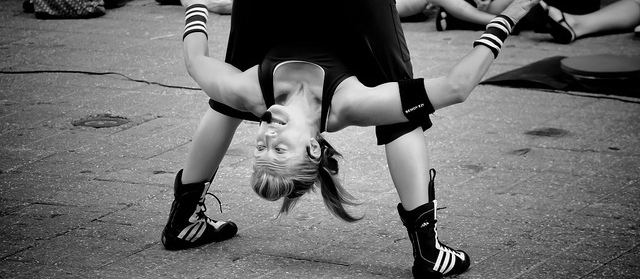
\includegraphics[width=4.8 cm]{images/hindsight-grey.jpg}};


  % \tikz{\fill (0,0) rectangle
  %   (\cardwidth-\strippadding-\stripwidth-2*\textpadding,\ruleheight);}\\
  % {\captionfontsize \bottomcaption}\\ {\textfontsize \bottomcontent}\\

\end{tikzpicture}

\end{document}
%%% Local Variables:
%%% mode: latex
%%% TeX-master: t
%%% End:
